% !TEX root = ../PhD Thesis.tex
\chapter{CompBio app server}
\label{chap:app-server}

Since I started building psichomics, I wanted my work to be publicly available as an online web app, providing users the most up-to-date version at their fingerprints, without having to install, update and manage different versions of R, Bioconductor, psichomics and all their dependencies.
%It can take an hour to install psichomics from scratch and the command line may scare the end-users for whom psichomics was created. 
Five years after the first Bioconductor release of psichomics in 2016, that vision finally came true.

\begin{figure}[!b]
  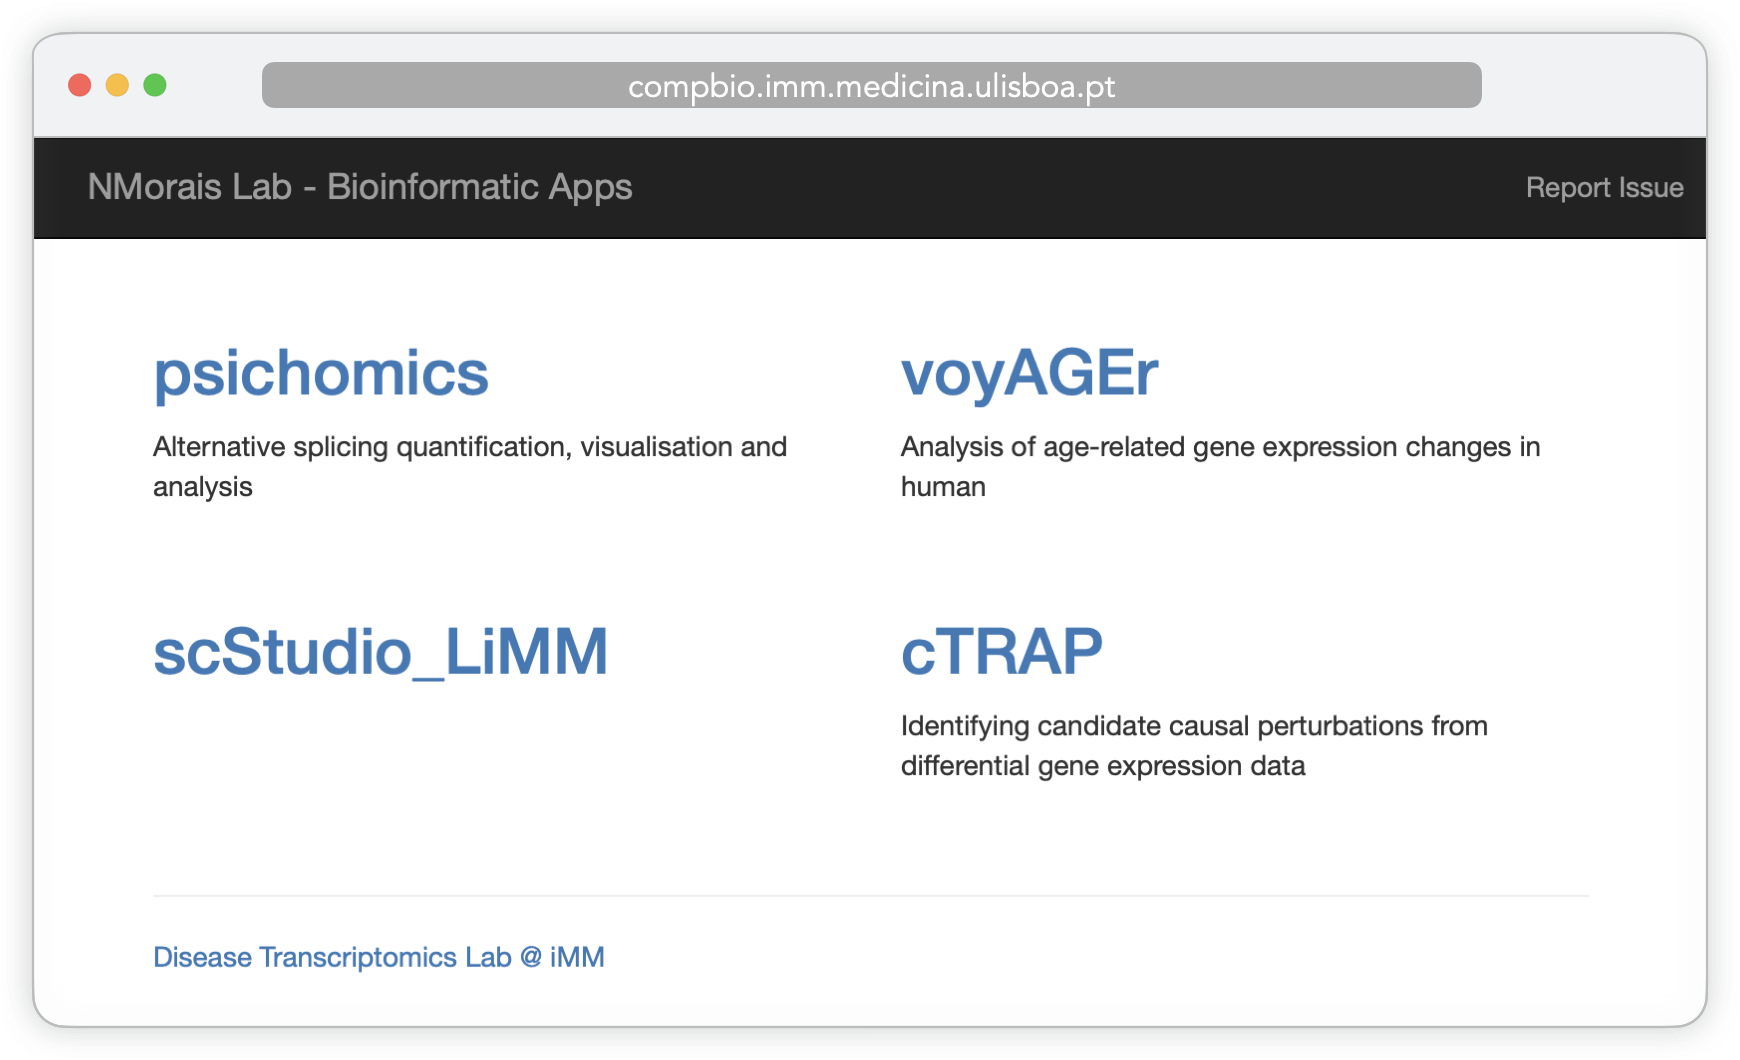
\includegraphics[width=.89\textwidth]{images/app-server/homepage}
  \centering
  \caption[Screenshot of CompBio's homepage]{\textbf{CompBio's homepage screenshot.} List of hosted web apps (11 Nov 2021).}
  \label{fig:homepage}
\end{figure}

One of our lab's ambitious goals is to develop interactive visual tools to assist in exploring biological data, either provided by users or available from big datasets. We want our tools to be used by anyone, no matter their computational background. To turn that dream into reality, I set up the CompBio app server, a Linux virtual machine running in iMM computing cluster that hosts psichomics, cTRAP and other Shiny apps from my lab colleagues. The server is accessible at \alink{compbio.imm.medicina.ulisboa.pt} (\autoref{fig:homepage}) and its code at \alink{github.com/nuno-agostinho/compbio-app-server}.

% TODO: write specs of the app server? 200GB SSD, 64GB RAM, 16 CPU threads

\section{Background}

Our lab uses the R statistical language to analyse clinical and molecular data from public sources and collaborators. In order to share data insights with our collaborators or even the whole scientific community, we have been increasingly creating exploratory dashboards using the Shiny R package \cite{chang:2021ul}. While developing interactive Shiny web apps, it is natural to wonder: what is the best way to share them?

\subsection{Desktop apps}

Shiny apps are written in R, an interpreted programming language whose source code can run in multiple platforms \cite{r-core-team:2021wf,chang:2021ul}. When run locally, the Shiny app starts running in the device itself (\texttt{localhost}) and is accessible via a web browser. Shiny apps can be part of an R package and be provided in CRAN or Bioconductor (such as in the case of psichomics and cTRAP). Nonetheless, this requires the user to install multiple programs in their computer: R, Shiny, the Shiny app, and all their dependencies. This can take up some time if the user does not have R and many of the required libraries installed. For instance, installing psichomics in a new system can take up to 1 hour. Moreover, it still requires opening an R session to start the visual interface, which may discourage technically-challenged users to try out psichomics.

% Java (\alink{java.com}) is a platform-independent, general-purpose programming language intended to allow the same code to target multiple platforms. It uses an intermediary Java virtual machine (JVM) that translates Jave bytecode to the native platform's language. On the other hand, graphical interfaces in Java can consume more time and memory than native apps, besides having a user interface that is in stark contrast to the graphical interface of other apps.

One way to reduce the number of dependencies installed is by using Docker (\alink{docker.com}), allowing to run isolated Linux virtual environments (containers) that already contain programs and all their dependencies set up. This approach simply requires end-users to install Docker and to download the desired Docker images online. Still, Docker is a program that needs administrator privileges for installation that (1) not all users may have and (2) may not feel comfortable to give to a software they would not otherwise install.

An alternative is Electron (\alink{electronjs.org}), a software framework that allows to develop cross-platform graphical user interface apps using web technologies by combining a web browser rendering engine (Chromium, used in Chrome and other web browsers to convert HTML and CSS code into an interactive web page) and a JavaScript environment. The app itself runs the web app as if it were a usual desktop app. Some open-source projects like electricShine (\alink{github.com/chasemc/electricShine}) and photon (\alink{github.com/COVAIL/photon}) allow to convert Shiny apps to Electron apps, but they are still not fully developed and lack important features (like support for some operative systems). Regardless, compared to native apps, Electron apps are slower, have a significant overhead, take more space and consume more RAM, making Electron less attractive for intensive data-processing apps.

\subsection{Web apps}

Web apps are cross-platform, always up-to-date and can be accessed by any (modern) web browser, making access to such apps easier for end-users \cite{silva:2017wl}. However, a constantly online web server needs to be running and share its computing resources (e.g. amount of RAM, storage and CPU threads) across multiple users. The resources allocated to a web server depend on the resources consumed per app, the number of simultaneous users and the data stored per user. The price of components and their maintenance is specially relevant if anticipating a large number of end-users.

Multiple web app hosting services support Shiny apps or Docker containers of Shiny apps, including Heroku (\alink{heroku.com}) and \alink{shinyapps.io}. Both of these app hosting services offer subscription plans depending on allocated system resources, including a free plan useful to run basic apps: Heroku's free plan offers 2 threads, 512 MB of RAM and 500 MB of storage per app\footnote{According to Heroku (\alink{heroku.com/pricing} and \alink{devcenter.heroku.com/articles/limits}) as of 24 November 2021. Unverified accounts (i.e. not associated with a valid credit card) are limited to 5 apps.}, whereas \alink{shinyapps.io}'s free plan allows for 5 apps with 25 computing hours per month using 1024 MB of RAM and 1 GB of storage per app\footnote{According to official \alink{shinyapps.io} documentation (\alink{docs.rstudio.com/shinyapps.io/applications.html} and \alink{shinyapps.io\#pricing}) as of 24 November 2021.}. Such services take care of deploying the web apps and we can select a different plan to scale up the required resources to run the apps, depending on their usage. They also allow to monitor app resource usage and understand how the apps are being used and if the resources employed are sufficient or not without much effort to the developer.

Besides third-party server hosting, Shiny apps can also be deployed in local web servers. This requires server maintenance and may be harder to scale resources because of higher up-front costs. The following programs allow to host Shiny apps in a local machine:

\begin{itemize}
	\item \textbf{Shiny Server} (\alink{rstudio.com/products/shiny/shiny-server}) is a bare-featured open-source program with only the essential features to host Shiny apps.
	\item \textbf{RStudio Connect} (\alink{rstudio.com/products/connect}) is a paid program\footnote{According to RStudio (\alink{rstudio.com/pricing}), all RStudio commercial products are free for teaching purposes and 50\% discounted for academic research from their regular bundle pricing starting at 22000\$ per year as of 24 November 2021.} with many more features than Shiny Server, including user authentication, Python-based app support and resource usage metrics.
	\item \textbf{ShinyProxy} (\alink{shinyproxy.io}) is an open-source program to host Shiny apps in Docker containers with many of the features found in RStudio Connect, including user authentication, Python-based app support and resource usage metrics.
\end{itemize}

Given that we have sufficient computing resources at our lab's disposal, we decided to build an app server -- a web server dedicated to deploy our web apps. We decided to use ShinyProxy as it has many of the advantages of using the proprietary RStudio Connect for free. Following this choice, we had to think how to properly develop the web server so it is easy to maintain, update and add new apps.

% Nginx as reverse proxy to handle all requests, including SSL certificates for HTTPS
% Nginx as a reverse proxy, serves as an intermediary between the user requests and the server.

In this chapter, I describe CompBio, our app server built with Docker Compose, a program to simultaneously manage multiple interacting Docker containers to allow for R/Shiny and Python app deployment (ShinyProxy) over a reverse proxy (Nginx), background tasks (Celery, Redis and Flower), website analytics (Plausible, PostgreSQL and ClickHouse), resource monitoring (Prometheus and Graphana), and feature testing (RStudio Web, only used to develop features and R scripts). CompBio is currently running in a virtual machine in a Linux computing cluster and hosts Shiny apps from NMorais lab, including the tools previously mentioned in this document: psichomics and cTRAP. CompBio is so named because it powers \textbf{Comp}utational \textbf{Bio}logy apps.

\section{Materials and methods}

CompBio is built using Docker Compose to manage the Docker images of multiple services: ShinyProxy, Nginx, Celery, Redis, Flower, Plausible, PostgreSQL, ClickHouse, Prometheus, Grafana and RStudio Web (\autoref{tab:compbio-services}). 
RStudio Web is only available in the development profile. The services communicate between each other via a single network created by Docker (\autoref{fig:architecture}).

\begin{table}[!ht]
\small
\caption[CompBio web services]{\textbf{CompBio web services.}}
\label{tab:compbio-services}
\begin{tabularx}{\textwidth}{ l l l }
\toprule
\parnoteclear
\textbf{Role}                    & \textbf{Service} & \textbf{Docker image}\parnote{Available in Docker Hub, unless stated otherwise.} \\
\toprule
Web app deployment                   & ShinyProxy       & \dockerlink{openanalytics/shinyproxy}     \\ \midrule
Reverse proxy                        & Nginx            & \dockerlink[_]{nginx}     \\ \midrule
\multirow{3}{6cm}{Background tasks} & Celery + cTRAP   & Based on \dockerlink{nunoagostinho/ctrap}\parnote{Python and Celery are installed on top of cTRAP Docker image, allowing Celery to run cTRAP analyses: see file \link{https://github.com/nuno-agostinho/compbio-app-server/blob/main/celery/Dockerfile}{celery/Dockerfile}.} \\
                                     & Redis            & \dockerlink[_]{redis}     \\
                                     & Flower           & \dockerlink{mher/flower}     \\ \midrule
\multirow{3}{6cm}{Website analytics
\par(i.e. track visitor metrics)}    & Plausible        & \dockerlink{plausible/analytics}     \\
                                     & PostgreSQL       & \dockerlink[_]{postgres}     \\
                                     & ClickHouse       & \dockerlink{yandex/clickhouse-server}     \\ \midrule
\multirow{2}{6cm}{Register and monitor
\par server resources}               & Prometheus       & \dockerlink{prom/prometheus}     \\
                                     & Grafana          & \dockerlink{grafana/grafana}     \\ \midrule
Run R sessions and test features     & RStudio Web\parnote{Only available in the development profile.} & Based on \dockerlink{rocker/rstudio} \\
\bottomrule
\end{tabularx}
\parnotes
\end{table}

\begin{figure}[!t]
  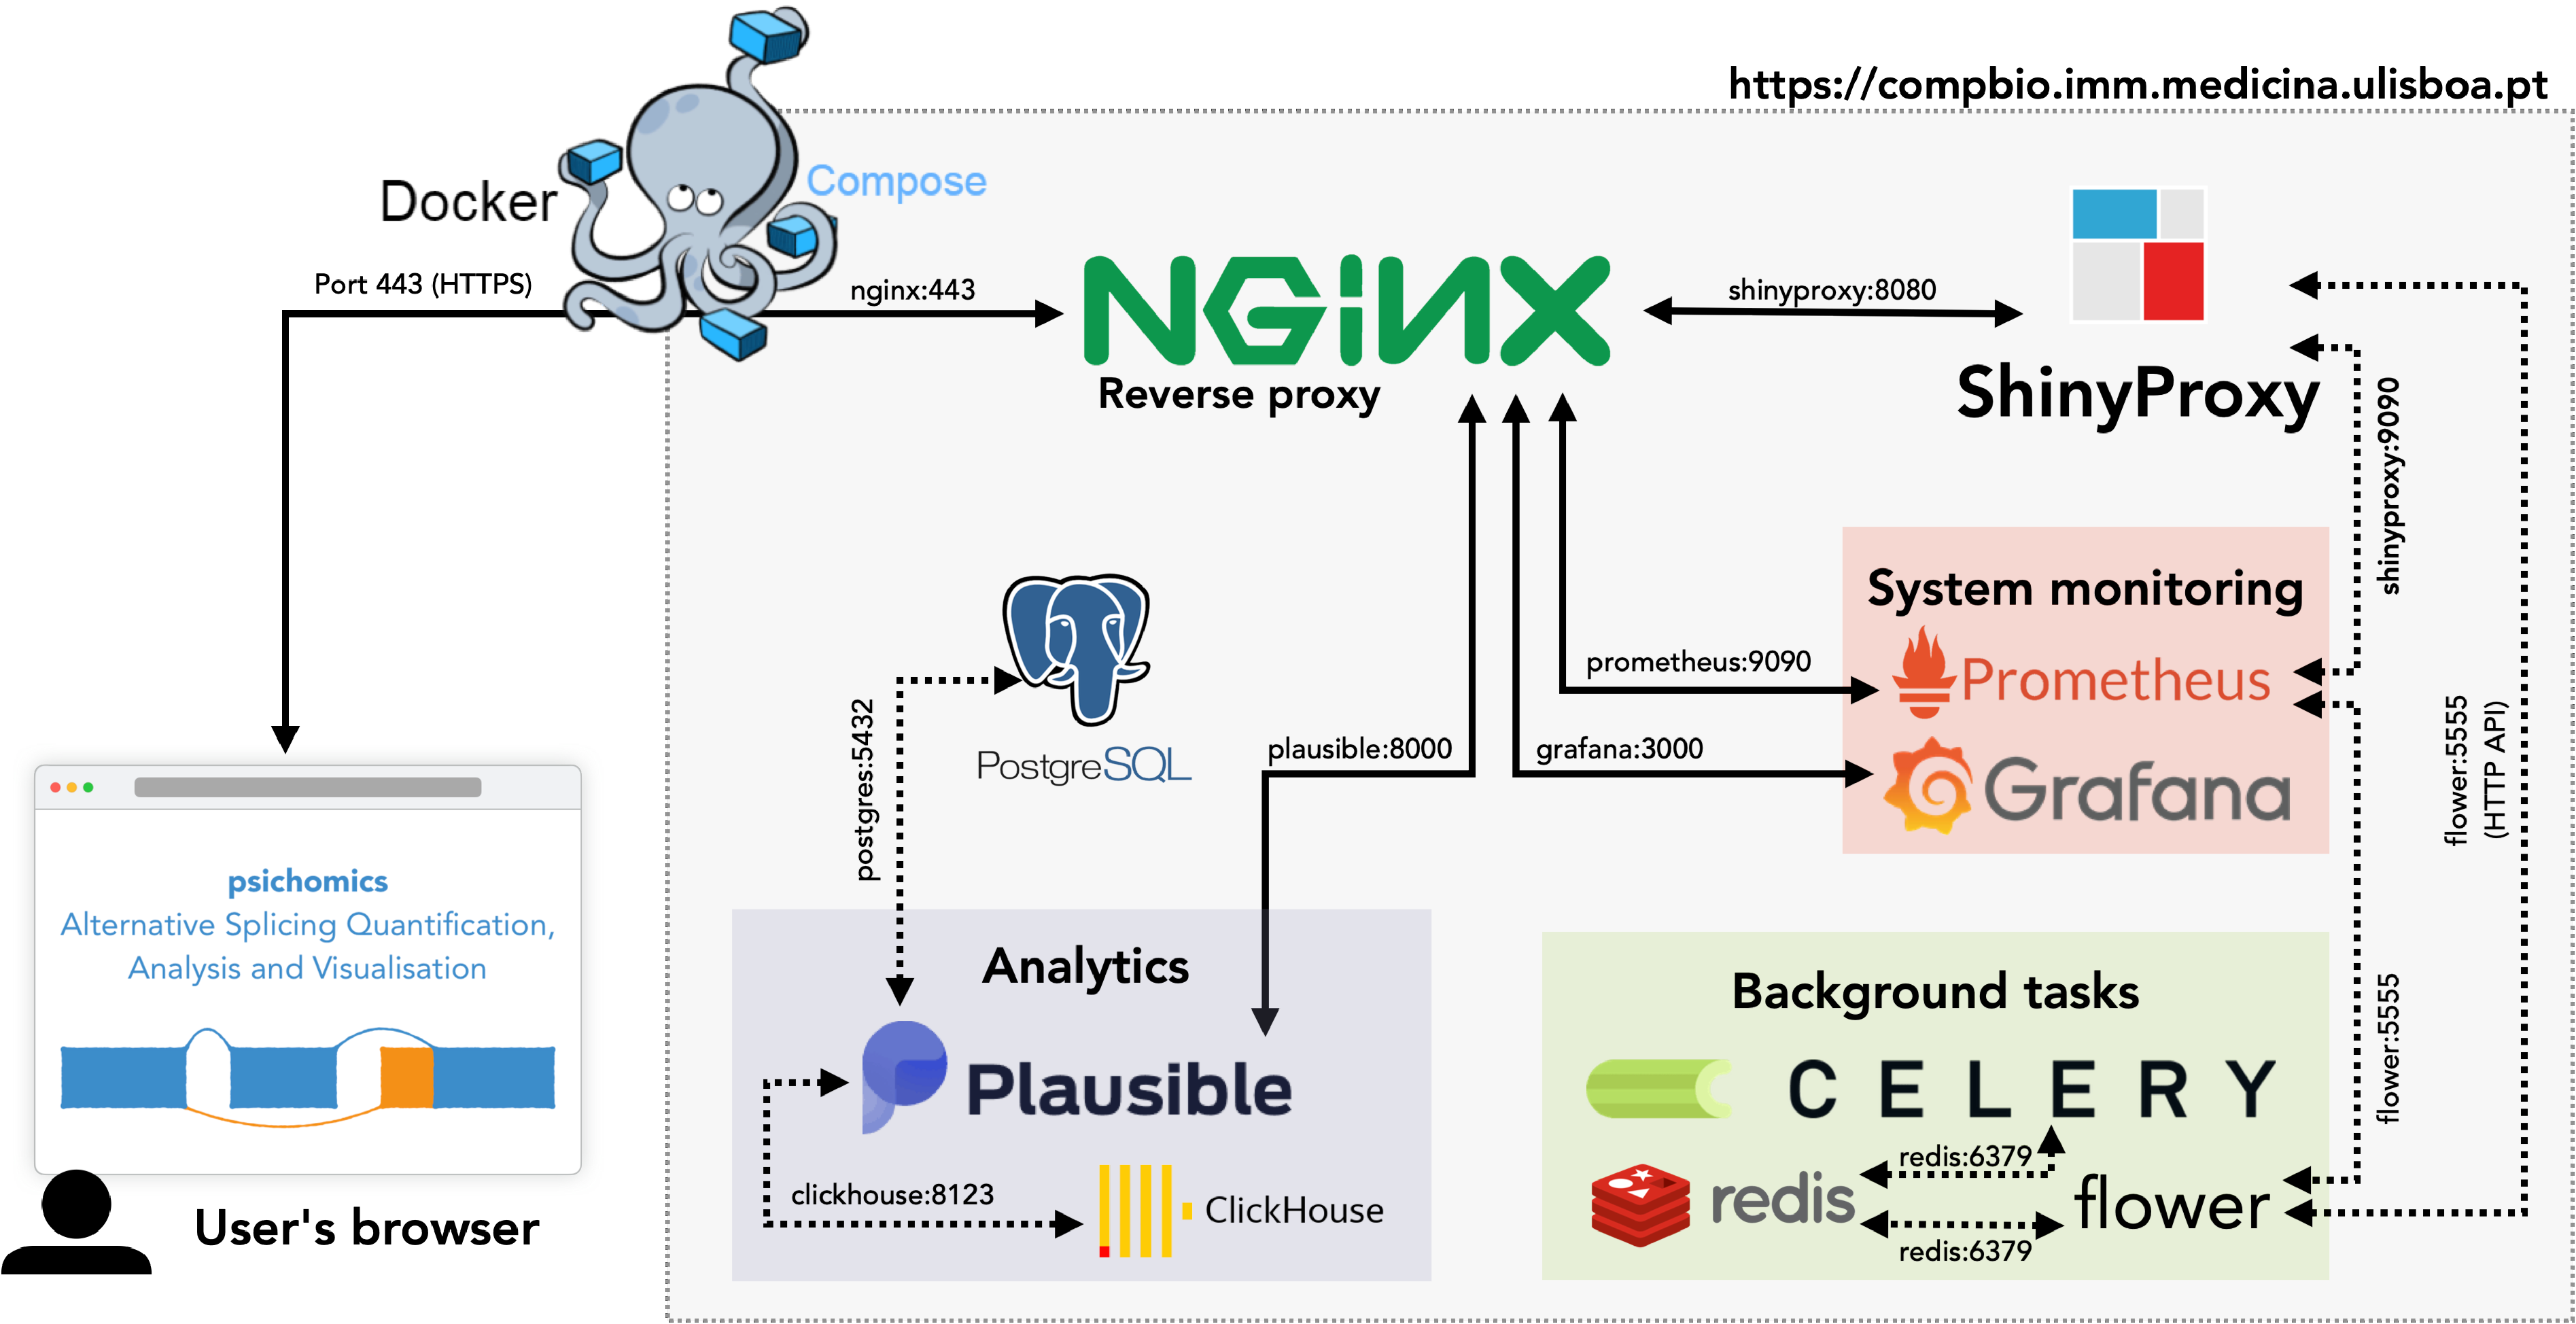
\includegraphics[width=.9\textwidth]{images/app-server/architecture}
  \centering
  \caption[App server architecture]{\textbf{App server architecture is based on Docker Compose.} All services are provided via Docker images and communicate with each other via a Docker-created network using the name of the service and a specific port (e.g. Nginx communicates with ShinyProxy via \texttt{shinyproxy:8080}). The groups  (analytics, system monitoring and background tasks) are strictly conceptual.}
  \label{fig:architecture}
\end{figure}

\section{Results}

The CompBio project makes use of a two-tiered architecture as the user interface is displayed using the user's web browser to render the HTML, CSS and JavaScript code, whereas the application and database layers are all run in the app server. %A disadvantage of this solution is that, if the app server is being heavily used, the database part is also slowed down. As the database is only being used

The code to run the CompBio app server supports Linux\footnote{CompBio may run in other operating systems. However, this is beyond the scope of this project.} machines with only Docker and Docker Compose installed, thus making the setup easily portable across different Linux computers and requiring minimal user setup.

\subsection{Design decisions}

The functional requirements for the app server were the following:

- Add new and update existing Shiny apps

- Easy to maintain and update

- Allow to run background processes (support for cTRAP long-running tasks)

- Track simple visitor metrics (e.g. apps used, elapsed time, geographical location of users, etc.)

- Monitor system usage

Noted non-functional requirements (quality attributes) for the app server include:

- Modular and maintainable (system components should be easy to update and replace without affecting other components)

- Extendable (easy to test new system components and deploy new apps)

- Scalable (support increasing/decreasing availability of system resources)

- Easy-to-use (easy to navigate and descriptive in case of errors)

- Open-source and free

- Portable

There are a lot of programs that can go into a web server. Experimenting different programs while managing their manifold dependencies to develop an healthy web server is like an intricate ballet where all finely-coordinated dancers interplay for an astounding performance. This can be as difficult as it sounds: a wrong move can affect the whole show. After all, each program/dependency has its own requirements and some may be a distress to (un)install. Moreover, when the server is online, errors may arise due to configuration changes (such as new app updates), requiring a fast rollback to minimise server downtime. A solution is to use self-contained and modular programs, such as in the case of Docker containers. But how to coordinate several Docker containers to beautifully perform the Swan Lake?

With Docker Compose, multiple applications are run isolated from others in their own Docker containers, allowing to easily update or replace them without affecting other system components. All services spawned in Docker Compose are Docker images, either pre-created (e.g.  Docker images from Docker Hub) or built before starting up all services (in this case, a Dockerfile is required to create the Docker images). Docker Compose allows to quickly play and swap programs: the services present in the server were selected after trying out many other combinations of alternative apps. The modularity of Docker Compose allows to easily test new system components and update software versions.

\subsection{Docker Compose}

All the code required to run the app server is available at \alink{github.com/nuno-agostinho/compbio-app-server}. A single file (\texttt{docker-compose.yml}) contains the main configuration of each application in the server, and extra configuration files are available in the local directory. For organisation purposes, the project is organised by folders named after each service, where each folder stores files (e.g. Dockerfile, configuration and data) associated with the respective application (\autoref{fig:file-structure}).

\begin{figure}[!ht]
  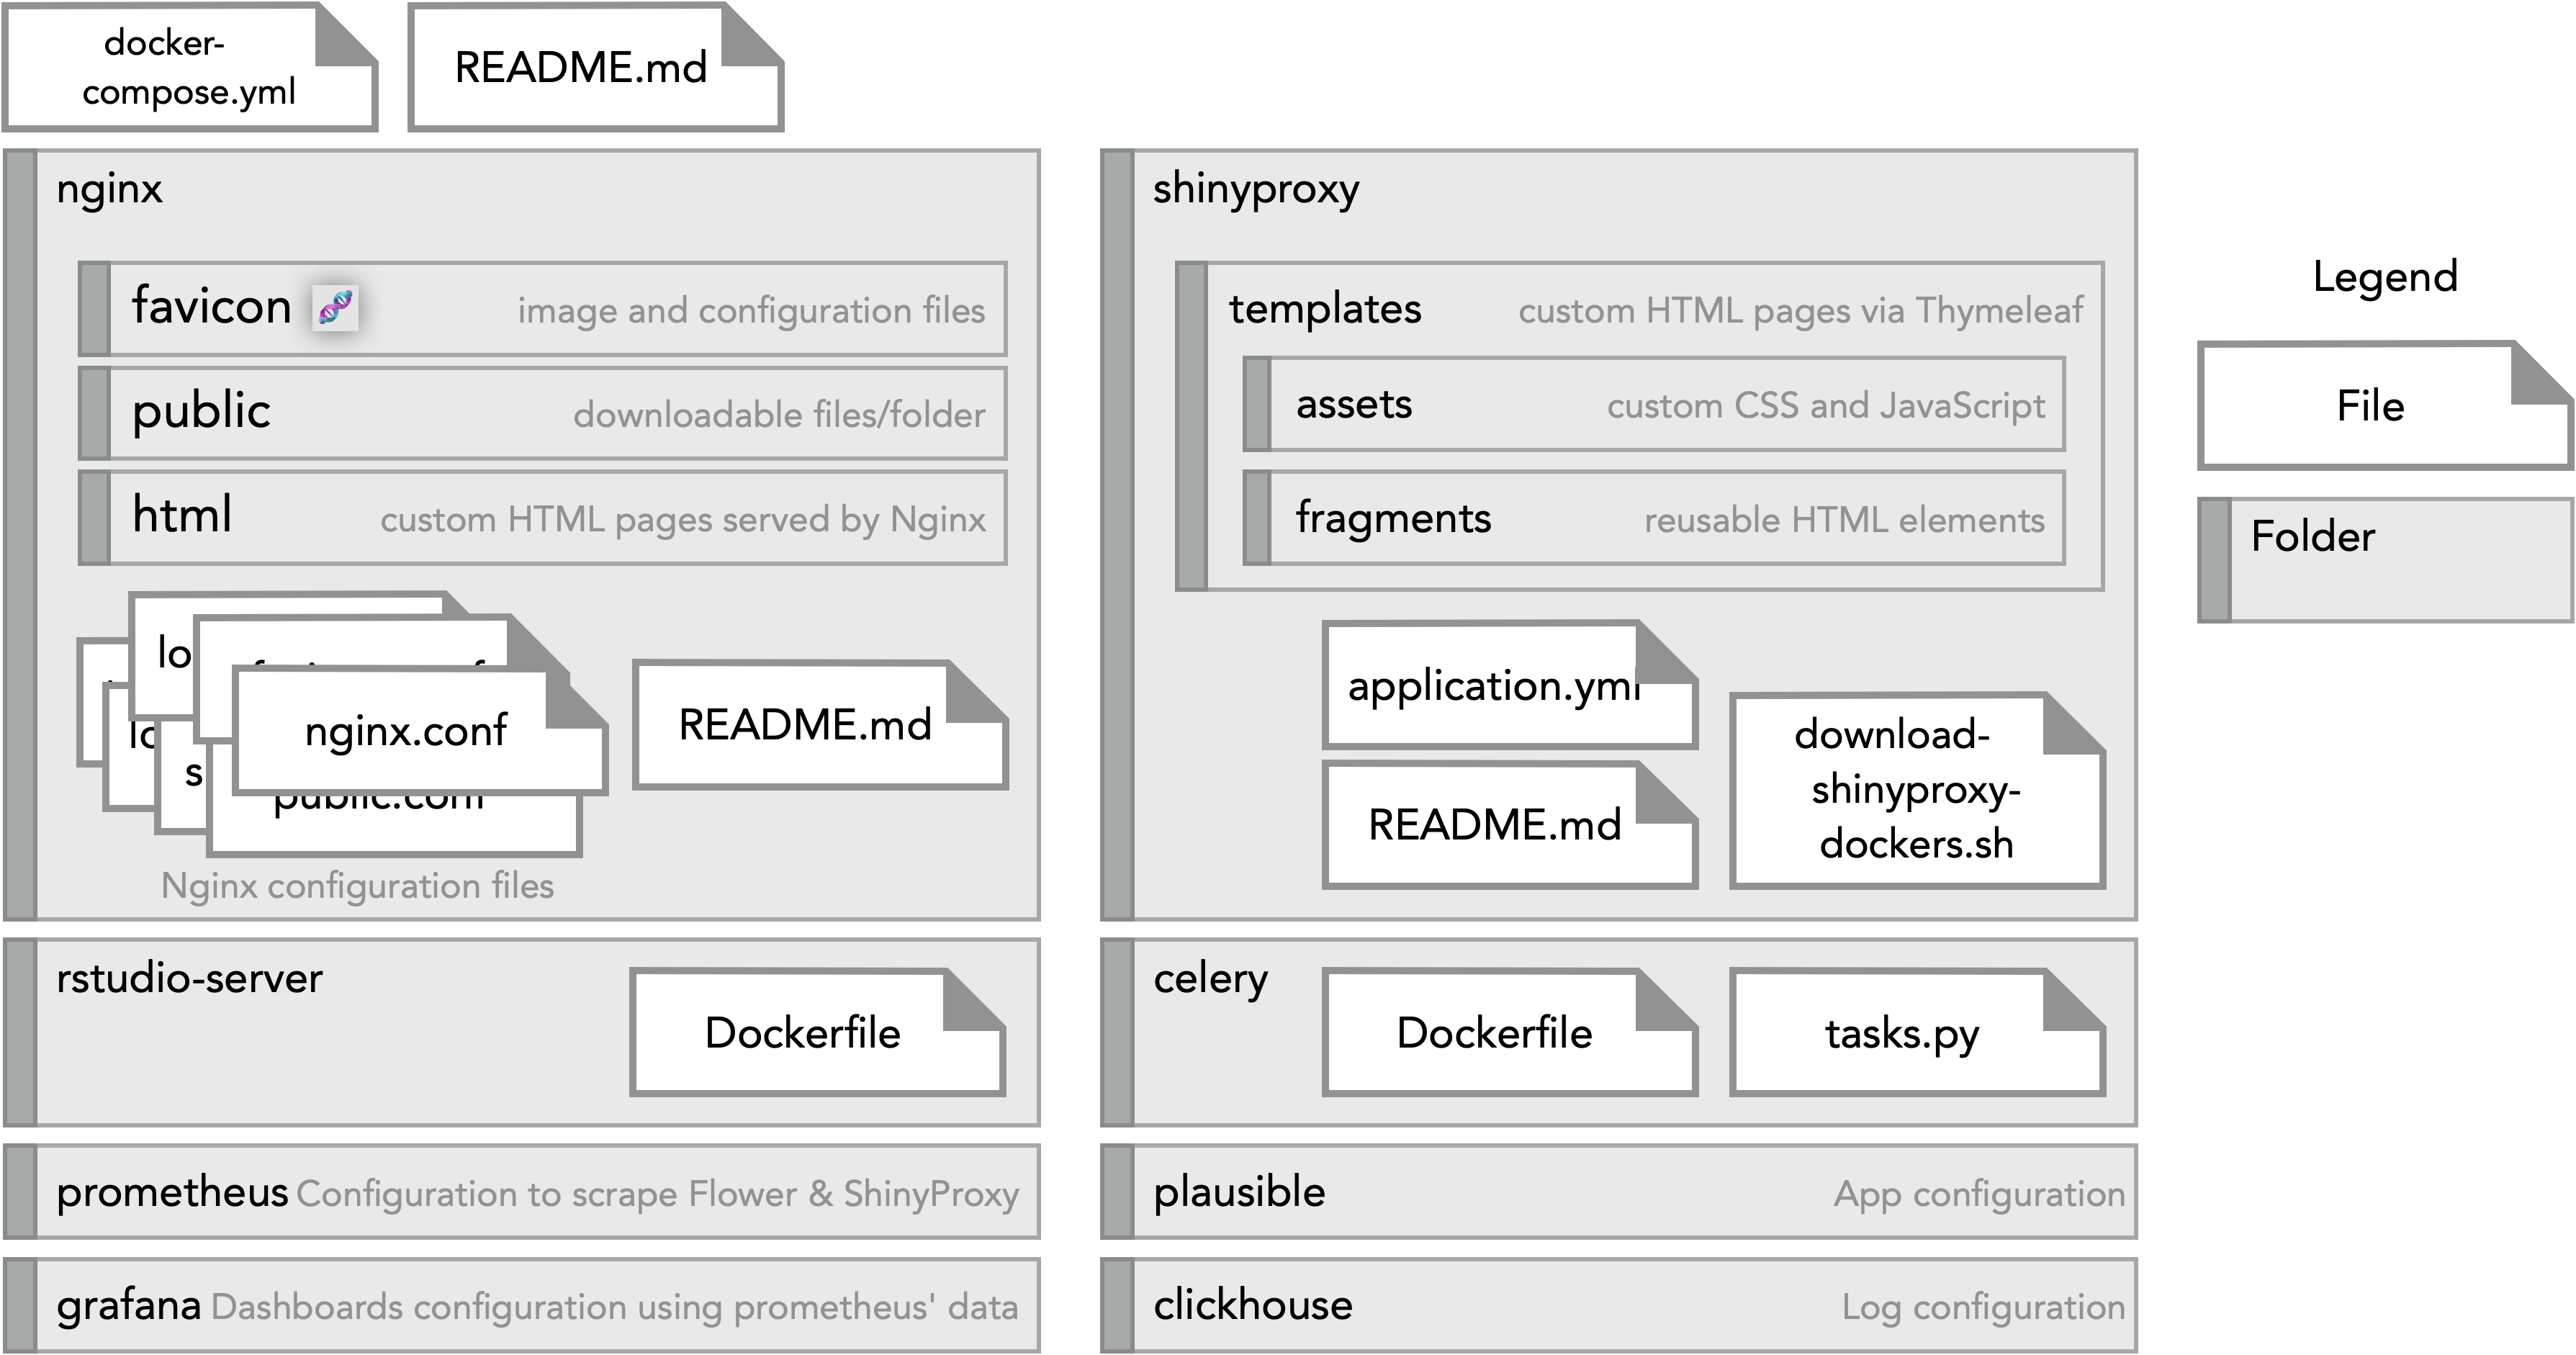
\includegraphics[width=1\textwidth]{images/app-server/file-structure}
  \centering
  \caption[App server's file structure]{\textbf{Visual representation of the file structure of the CompBio app server.} Each folder contains files associated with a specific service. Folders \texttt{rstudio-server} and \texttt{celery} contain Dockerfiles for building custom Docker images of the respective services. Multiple \texttt{README.md} document the usage of the services and the app server itself. The root file \texttt{docker-compose.yml} contains the main configuration of each service.}
  \label{fig:file-structure}
\end{figure}

The command \texttt{docker-compose up -d --build} downloads Docker images mentioned in \texttt{docker-compose.yml}, builds Docker images from Dockerfiles (argument \texttt{--build}) and starts up the services in detached mode (argument \texttt{-d}).

Although data from Docker containers are only available temporary after the container is stopped, files can be preserved in Docker volumes to avoid data loss when restarting services. When starting the \texttt{docker-compose.yml} project, Docker volumes for specific directories (e.g. database data) are mounted.

Docker Compose has multiple commands to manage the services. For instance, it is possible to restart single services without affecting other programs, like \texttt{docker-compose restart shinyproxy}. This is useful after modifying the configuration of a service. However, changes to \texttt{docker-compose.yml} are only applied when shutting down all services with \texttt{docker-compose down}.

% kubernetes?
% Ansible?

\subsection{ShinyProxy}

ShinyProxy is an open-source program that deploys R/Shiny and Python apps via Docker. When a user starts an app, ShinyProxy creates a new Docker container exclusively for that user. The containers are automatically terminated 30 minutes (by default) after the last user interaction.

Deploying new Shiny apps in the app server is as simple as adding the name of the Docker image in the ShinyProxy configuration file (\texttt{shinyproxy/application.yml}), downloading the respective Docker image and restarting ShinyProxy. Alternatively, running the script \texttt{download-shinyproxy-dockers.sh} automatically downloads or updates Docker images used in ShinyProxy.

ShinyProxy offers multiple built-in features, including:

\begin{itemize}
    \item \textbf{App recovery:} when restarting ShinyProxy, ShinyProxy-initiated Docker containers continue running in the background. The apps will be unavailable while ShinyProxy is not running, but will be attached to ShinyProxy once it is running again, allowing for quick server maintenance tasks\footnote{More information in \alink{shinyproxy.io/documentation/app-recovery}.}.
    \item \textbf{User authentication:} authentication with multiple methods, including social login via GitHub, LinkedIn, Google, etc. However, user authentication requires all visitors to login before continuing. As we prefer users to be able to anonymously access our apps, this feature is currently disabled.
%    \item \textbf{User sessions:} user data can be stored in user-specific folders. As the sessions are only accessible when the Docker container is already attached to the volumes, this allows for complete isolation from other user folders. This feature works best with user authentication enabled (otherwise, random identifiers are used for each visitor and requires custom logic to load data between computers).
	\item \textbf{Multiple app instances:} users can open and manage multiple app instances simultaneously (not currently enabled in the app server)\footnote{More information in \alink{shinyproxy.io/documentation/ui/\#using-multiple-instances-of-an-app}.}.
\end{itemize}

\subsubsection{Progress bar when loading ShinyProxy apps}

\begin{wrapfigure}{r}{.5\textwidth}
  \vspace{-\intextsep}
  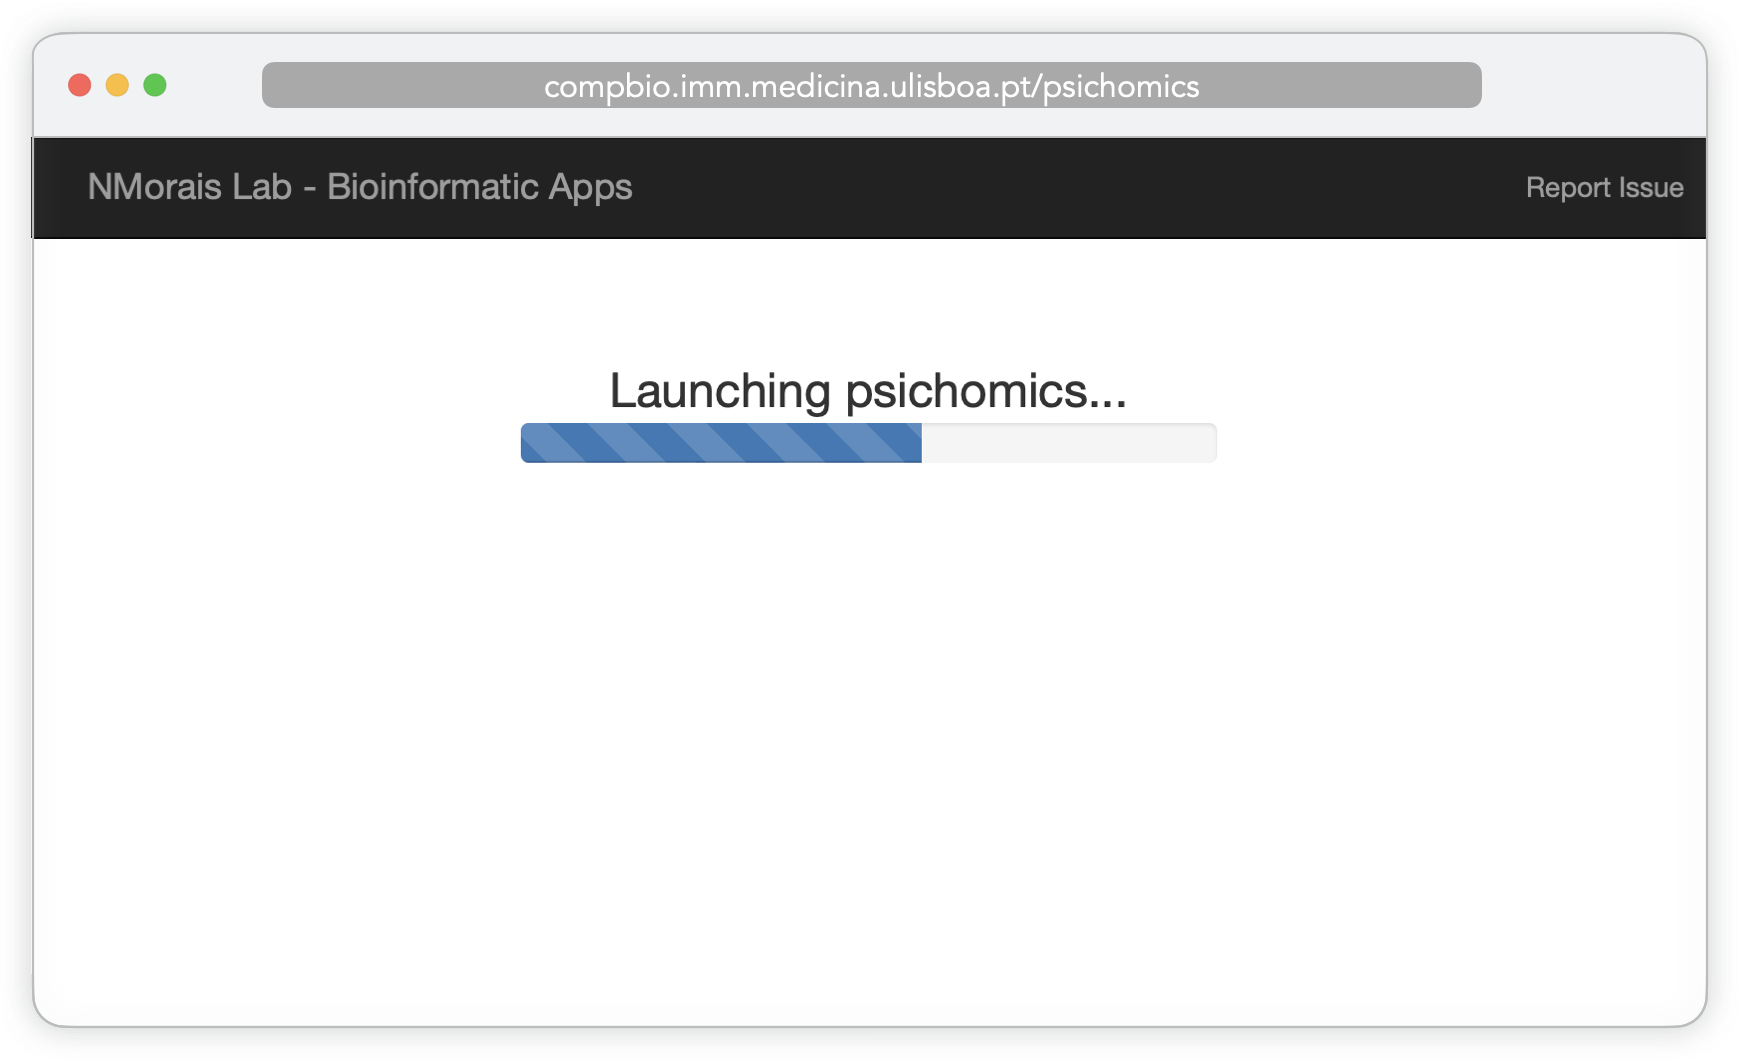
\includegraphics[width=\linewidth]{images/app-server/progress-bar}
  \caption[Screenshot of app loading]{\textbf{Progress bar displayed while psichomics loads} (11 Nov 2021).}
  \label{fig:progress-bar}
  \vspace{-\intextsep}
\end{wrapfigure}

% https://dl.acm.org/doi/pdf/10.1145/1294211.1294231
% https://www.chrisharrison.net/index.php/Research/ProgressBars2
% https://dl.acm.org/doi/pdf/10.1145/2702123.2702139
% https://www.researchgate.net/publication/234791131_The_importance_of_percent-done_progress_indicators_for_computer-human_interfaces
% https://ieeexplore.ieee.org/stamp/stamp.jsp?tp=&arnumber=6263888&tag=1

When ShinyProxy is loading an app, a spinning wheel is shown as a loading indicator. For apps that take more than 10 seconds to load (e.g. psichomics and cTRAP), the user may think the website is not working and close the window before the app is loaded. To avoid that, the spinning wheel was replaced with a progress bar to provide a time estimate for app loading (\autoref{fig:progress-bar}), making wait times more tolerable \cite{myers:1985us,yablonski:2020ts}.

By default, the progress bar takes 5 seconds to fill (as sample Shiny apps take that much to launch in ShinyProxy), but the time is customisable for specific apps by editing the ShinyProxy configuration file (\texttt{shinyproxy/application.yml}) and adding a \texttt{template-properties.start-up} parameter to a specific app. For instance, psichomics takes 20 seconds to fully load the progress bar (i.e. \texttt{template-properties.start-up: 20s}), whereas cTRAP takes 15 seconds. When the app finishes loading, the progress bar is replaced by the app regardless of the progress displayed to the user. The accuracy of the progress bar does not have to be perfect to serve its purpose \cite{myers:1985us,yablonski:2020ts}.

%To create this progress bar, \verb|shinyproxy/templates/app.html| was edited to remove the spinning wheel and to include an empty progress bar. The progress bar's width is changed from 0\% to 100\% using JavaScript. By default, the CSS width transition applied to the progress bar is \texttt{transition: width 5s ease-in-out;} (animating a change of width that last for 5 seconds in an ease-in animation) where \texttt{5s} is replaced by the \texttt{template-properties.startup-time} parameter if set.

\subsubsection{Custom HTML pages}

\subsection{Nginx}

Nginx is a reverse proxy, i.e. an intermediary that decides what is shown to the user depending on the URL visited (akin to those switchboard operators seen in the old movies). In CompBio, Nginx is responsible to fulfil user requests, to ensure HTTPS traffic is encrypted via SSL certificates, serve publicly available files and show a custom error page if ShinyProxy is not responding (e.g. temporarily down or overloaded).

Nginx is also used for ensuring encrypted HTTPS traffic via SSL certificates. SSL certificates are handed by the IT team at iMM and we only need to point Nginx to the correct location of those certificates. SSL certificates include three separate parts: the site certificate, intermediate certificates, and the private key.

% public
A public folder is available via Nginx.

% custom HTML error page
In case ShinyProxy is down, Nginx will serve a custom error page stating that the server is down probably because of ShinyProxy. This is informative enough to end-users that know they should wait to refresh the page in a moment and also to admins that will understand that ShinyProxy is temporarily down (this can happen because of multiple reasons, such as a restart of the service or overloading).

% favicon

% An issue with Nginx is that it is especially verbose compared to more recent reverse proxies. Although I would have liked to replace Nginx with a simpler reverse proxy -- such as Caddy (\alink{caddyserver.com}) --, Nginx is more popular and widely used, thus making it easier to find documentation and to Google issues.

\subsection{Background tasks}

The main goal of our app server is to deploy Shiny apps, i.e. apps that were developed in R. The main disadvantage of using R is that it was designed for running single-thread processes. When running a Shiny app, that is specifically hard, as users cannot interact with the app while analysing data. This has been solved in multiple ways that extend R:

- by using promises/future

- by running R in the background

However, using any of those solutions implies that the Docker container needs to be active during the whole process, which can be especially egregious if the user session is big and is consuming many resources, disallowing other users to  use those resources.

But how to make large tasks run in the background? In Lobo, iMM's computing cluster, we use a task manager for that function: SLURM. However, SLURM is too complex to install -- I was not able to make a working prototype of SLURM with Docker Compose. So, what about a light-weight SLURM? That is what Celery is, a Python package that 

% Redis as database
% Flower for HTTP API + table
% How does it run R?

\subsection{Website analytics}

Plausible is an open-source, privacy-focused web analytics tool that collects traffic metrics for multiple websites and provides them via an interactive dashboard. CompBio runs the self-hosted version of Plausible. All of Plausible metrics (e.g., visitor numbers, total page views and session duration) are anonymously aggregated without cookies, thus avoiding individual tracing.

% plausible + clickhouse + postgres
% postgres can be used in the future as the SQL database of the server

% plausible vs google analytics
Using the self-hosted version of Plausible guarantees that the user data tracked is done locally in the server. Plausible also protects user privacy by making their data hard to individually trace and by complying with current privacy laws (GDPR, CCPA and PECR). This is in stark contrast with Google Analytics.

\subsection{Resource monitoring}

Prometheus monitors server resources. Graphana is used to visualise the metrics collected by Prometheus.

Celery % TODO: add Graphana screenshot

% TODO: add Graphana screenshot
Many ShinyProxy metrics (including app usage time, app failures and user numbers) are collected with Prometheus and visualised using Grafana.

Nginx requires further configuration to be monitored. Currently, it is not monitored. % TODO: add Graphana screenshot

System % TODO: add Graphana screenshot

\subsection{Server maintenance}

% TODO: Run Docker images as rootless
% TODO: Change service passwords

CompBio is a web server that hosts Shiny applications and is publicly accessible by everyone online. This makes our server a target for potential security attacks. In order to mitigate such vulnerabilities, it is crucial to update user-facing programs (Docker, Docker Compose, Nginx and ShinyProxy), while components that are not directly available to end-users should be updated when possible. As updates may contain breaking changes that hamper website functionality, it is recommended to read change logs related to new software versions to pinpoint potential issues before updating.

% https://www.sciencedirect.com/science/article/pii/S2352484721007289#b71
% https://doi.org/10.1145/3038923
% https://www.tandfonline.com/doi/full/10.1080/19393555.2020.1853855?casa_token=EpT3lJflBXAAAAAA%3AaS5ePDNIcAPfL6MsMoKrI0s4sDtjyGNvGICZiz2Ywvnf7E2vtokORb073GUi9eilZiUCFOAqhIY

Updates to Docker and Docker Compose need to be performed by an administrator using Linux's \texttt{apt-get} command\footnote{sudo apt-get update \&\& sudo apt-get upgrade}. Docker images of the server (including Nginx and ShinyProxy), on the other hand, require a user in the \texttt{docker} group to edit the versions of the Docker images used in \texttt{docker-compose.yml} and restart the Docker Compose project\footnote{While inside the project folder: \texttt{docker-compose down \&\& docker-compose up -d --build}}. The advantage of using Docker Compose: if something goes wrong with the updated Docker images, simply revert \texttt{docker-compose.yml} to a previous working state and restart.

% root + Docker?

\section{Conclusion}

I think that the requirements for the app server were met with the current implementation.

CompBio currently runs in a virtual machine in Lobo, iMM computing cluster. All the hardware-related issues are taken care by the iMM IT team and they also support us with issues regarding SSL certificates, WebSocket connections and resource allocation. Moreover, I expect the server components to be easy to maintain and update. Components need to be manually updated but, in case of issues, it is easy to rollback to a stable, working version of the app server with previously used Docker images.

In the future, we can increase resources of our virtual machine if needed. In case we prefer to port the app server to a new machine, as the project was built on Docker Compose, relocating the app server is as easy as moving the project data to the new machine, installing Docker and Docker Compose, downloading required Docker images and starting the app server as previously indicated.

% Future updates
